\let\negmedspace\undefined
\let\negthickspace\undefined
\documentclass[journal]{IEEEtran}
\usepackage[a5paper, margin=10mm, onecolumn]{geometry}
%\usepackage{lmodern} % Ensure lmodern is loaded for pdflatex
\usepackage{tfrupee} % Include tfrupee package

\setlength{\headheight}{1cm} % Set the height of the header box
\setlength{\headsep}{0mm}     % Set the distance between the header box and the top of the text

\usepackage{gvv-book}
\usepackage{gvv}
\usepackage{cite}
\usepackage{amsmath,amssymb,amsfonts,amsthm}
\usepackage{algorithmic}
\usepackage{graphicx}
\usepackage{textcomp}
\usepackage{xcolor}
\usepackage{txfonts}
\usepackage{listings}
\usepackage{enumitem}
\usepackage{mathtools}
\usepackage{gensymb}
\usepackage{comment}
\usepackage[breaklinks=true]{hyperref}
\usepackage{tkz-euclide} 
\usepackage{listings}
% \usepackage{gvv}                               

\def\inputGnumericTable{}                      
\usepackage[latin1]{inputenc}                    
\usepackage{color}                              
\usepackage{array}                             
\usepackage{longtable}                          
\usepackage{calc}                               
\usepackage{multirow}                           
\usepackage{hhline}                            
\usepackage{ifthen}                          
\usepackage{lscape}
\begin{document}

\bibliographystyle{IEEEtran}
\vspace{3cm}

\title{1.3.2}
\author{AI25BTECH11023 - Pratik R
}
% \maketitle
% \newpage
% \bigskip
{\let\newpage\relax\maketitle}

\renewcommand{\thefigure}{\theenumi}
\renewcommand{\thetable}{\theenumi}
\setlength{\intextsep}{10pt} % Space between text and floats


\numberwithin{equation}{enumi}
\numberwithin{figure}{enumi}
\renewcommand{\thetable}{\theenumi}


\textbf{Question: }\\
The coordinates of the three consecutive vertices of a parallelogram $ABCD$ are
\textbf{A}$(1,3)$, \textbf{B}$(-1,2)$, and \textbf{C}$(2,5)$. Find the coordinates of the fourth vertex \textbf{D}.

\textbf{Solution: } \\
Given that
$$
\vec A = \myvec{1 \\ 3}, \vec B = \myvec{-1 \\ 2}, \vec C = \myvec{2 \\ 5}.
$$

The coordinates of $D$ of parallelogram $ABCD$ are obtained by equating midpoint of parallelogram:  

\begin{align}
\frac{\vec D + \vec B}{2} &= \frac{\vec A + \vec C}{2} \\
\vec D &= \vec A + \vec C - \vec B \\
\vec D &= \myvec{1 \\ 3} + \myvec{2 \\ 5} - \myvec{-1 \\ 2} \\
\vec D &= \myvec{4 \\ 6}
\end{align}

\begin{figure}[h!]
    \centering
    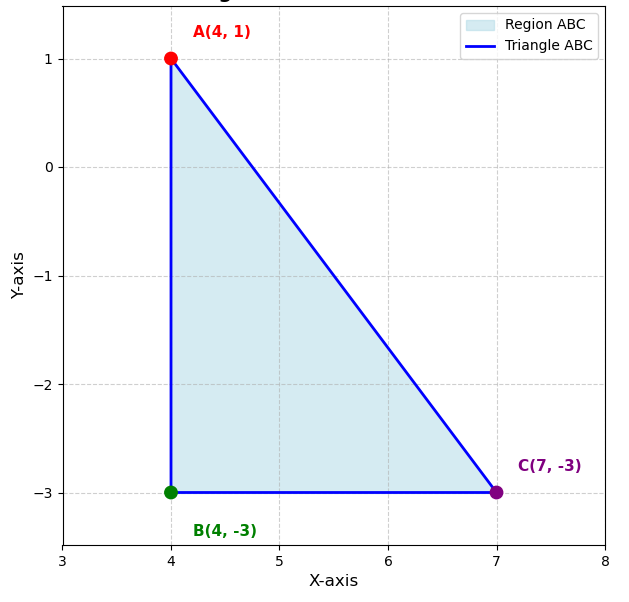
\includegraphics[width=0.7\columnwidth]{figs/fig.png}
    \caption{}
\end{figure}


\end{document}
